\documentclass[12pt, titlepage]{article}
\usepackage[shortlabels]{enumitem}
\usepackage{comment}
\usepackage{booktabs}
\usepackage{tabularx}
\usepackage{hyperref}
\usepackage{float}
\usepackage{soul}
\usepackage{changepage}
\usepackage{graphicx}
\setstcolor{red}
\hypersetup{
    colorlinks,
    citecolor=black,
    filecolor=black,
    linkcolor=black,
    urlcolor=blue
}
\usepackage[dvipsnames]{xcolor}
\usepackage[round]{natbib}

%% Comments

\usepackage{color}

\newif\ifcomments\commentstrue %displays comments
%\newif\ifcomments\commentsfalse %so that comments do not display

\ifcomments
\newcommand{\authornote}[3]{\textcolor{#1}{[#3 ---#2]}}
\newcommand{\todo}[1]{\textcolor{red}{[TODO: #1]}}
\else
\newcommand{\authornote}[3]{}
\newcommand{\todo}[1]{}
\fi

\newcommand{\wss}[1]{\authornote{blue}{SS}{#1}} 
\newcommand{\plt}[1]{\authornote{magenta}{TPLT}{#1}} %For explanation of the template
\newcommand{\an}[1]{\authornote{cyan}{Author}{#1}}

%% Common Parts

\newcommand{\progname}{ProgName} % PUT YOUR PROGRAM NAME HERE
\newcommand{\authname}{Team \#, Team Name
\\ Student 1 name
\\ Student 2 name
\\ Student 3 name
\\ Student 4 name} % AUTHOR NAMES                  

\usepackage{hyperref}
    \hypersetup{colorlinks=true, linkcolor=blue, citecolor=blue, filecolor=blue,
                urlcolor=blue, unicode=false}
    \urlstyle{same}
                                


\setcitestyle{numbers}

\title{SE 4G06: Software Requirements Specification\\\textit{Measuring Microstructure Changes During Thermal Treatment }}

\author{\authname}

\date{}

\begin{document}

\maketitle

\pagenumbering{roman}
\tableofcontents
\listoftables
\listoffigures

\begin{table}[H]
\caption{\bf Revision History}
\begin{tabularx}{\textwidth}{p{2.5cm}p{2.5cm}X}
\toprule {\bf Date} & {\bf Developer} & {\bf Notes/Changes}\\
\midrule
Sept 25, 2021 & Edwin Do & Revision 0 - Initial commit\\
Oct 5, 2021 & Edwin Do & Adopt Volere template + Add content \\
Oct 5, 2021 & Joseph Braun & Add functional Requirements \\ 

\bottomrule
\end{tabularx}
\end{table}

\newpage

\pagenumbering{arabic}

This document describes the software requirements for the capstone project of measuring microstructure changes of samples during thermal treatment. The template for the Software Requirements Specification (SRS) is a subset of the Volere
template.


\section{Project Drivers}

\subsection{The Purpose of the Project}
The purpose of this project is to assist the Department of Materials Engineering in measuring the changes to a material's microstructure during thermal treatment. 
By doing so, the resistivity of the sample can be measured at different thermal levels. The goal is to be able to collect the data at necessary sampling rate and 
incorporate the use of Windows GUI. 

\subsection{The Stakeholders}

\subsubsection{Developers}
The Developers will be responsible for the design, development, and documentation throughout. They will be utilizing the existing lab equipment, computer for the duration of this project.
Developers will also use the feedback from the client to deliver the final product. 

\subsubsection{The Client}
The Client for this project is the Department of Materials Engineering and the Computing and Software Department at McMaster University. More specifically, Dr. Zurob, Dr. Smith and TAs of 4G06 who will be the ones to evaluate, review and provide feedback on the project throughout the development process.

\subsubsection{The Customers}
The Customers for this project are anyone who will be conducting research or require data that measures the microstructural changes of materials under various thermal treatment.   

\subsubsection{Other Stakeholders}
This project has no other stakeholders.

\subsection{Mandated Constraints}

\subsubsection{Solution Constraints}

Description: The GUI will run on Windows operating system\\ 
Rationale: The application is a Desktop application. The lab computer that has the capability to connect to other required lab equipment currently runs on Windows.\\
Fit Criterion: Users can successfully install and open the application on a supported Windows operating system. \\

\noindent Description: The sampling rate of the equipment to the GUI will be at least 100 times per second\\ 
Rationale: According to Dr.Zurob, this is the minimum sampling rate needed to see any meaningful data\\
Fit Criterion: The equipment samples the data at 100 times per second and the GUI accurately reflects the measurements  \\

\subsubsection{Off-the-shelf Software}
No off-the-shelf software is required for this project. 

\subsubsection{Anticipated Workplace Environment}
The software and equipment will be designed for the expected environment of a lab. The reason is that the lab equipment and computer is needed for the software to run successfully and
should not be easily accessible outside of campus. 

\subsubsection{Schedule Constraints}
% Add other deadlines
The deadline for the final product is the March 20 2023. There will be other milestones during the development process that must be accomplished throughout. 
This will be outlined in our Github milestones.


\subsubsection{Budget Constraints}
% Double check this
At this point, there is an estimated budget of \$1000. This may change as the team determines what additional equipment is needed to work with the lab equipment.

\subsection{Naming Conventions and Terminology}

\begin{itemize}
    \item \textbf{JavaScript}: Scripting language used to create and control dynamic content.
    \item \textbf{HTML}: Standard markup language for creating web pages.
    \item \textbf{CSS}: Style sheet language for structuring and styling HTML web page.
    \item \textbf{Windows}: A popular operating system used by many users.
    \item \textbf{Product/Software/Application}: Refers to the final deliverable of this capstone project.
    \item \textbf{User}: The person who will be interacting/ using the application.
    \item \textbf{Electron}: JavaScript framework used to develop Desktop applications.  
\end{itemize}

\subsection{Relevant Facts and Assumptions}
\subsubsection{Facts}
ADD TEXT HERE
% Include a couple sentences about the background and maybe an equation describing how the conductivity is calculated.

\subsubsection{Assumptions}
ADD TEXT HERE
% Include a couple sentences about any assumptions that we have

\subsubsection{User Characteristics}
An assumption made about this project is that the users will have the necessary knowledge to safely operate the necessary lab equipment. This is required to collect the data and display it on the GUI. 
The user is also assumed to have general working knowledge of how to install and open a windows application, as well as the use of a mouse and keyboard input. Another assumption is that the user is literate in English.

\section{Functional Requirements}
\subsection{The Scope of the Work and the Product}

The hardware for this project is provided by the Department of Materials Engineering through the project supervisor, Dr. Zurob. A Windows computer, current source, and nanovoltmeter have already been included. A fourth hardware device, for measuring the temperature of the sample material, will also be provided or else a new device shall be purchased for this purpose. The product will be a Window's based GUI application which can set the data acquisition rate (sample rate), connect to the hardware devices, acquire the output data, and calculate the conductivity of the sample material in real time. The application should also be able to be accessed remotely to check on the progress of ongoing experiments. \\

\subsubsection{The Context of the Work}
% Electron - JS, HTML , CSS
% CI/CD - Build
% Devs may require the use of other libraries to speed up the dev process
\begin{figure}[H]
\centerline{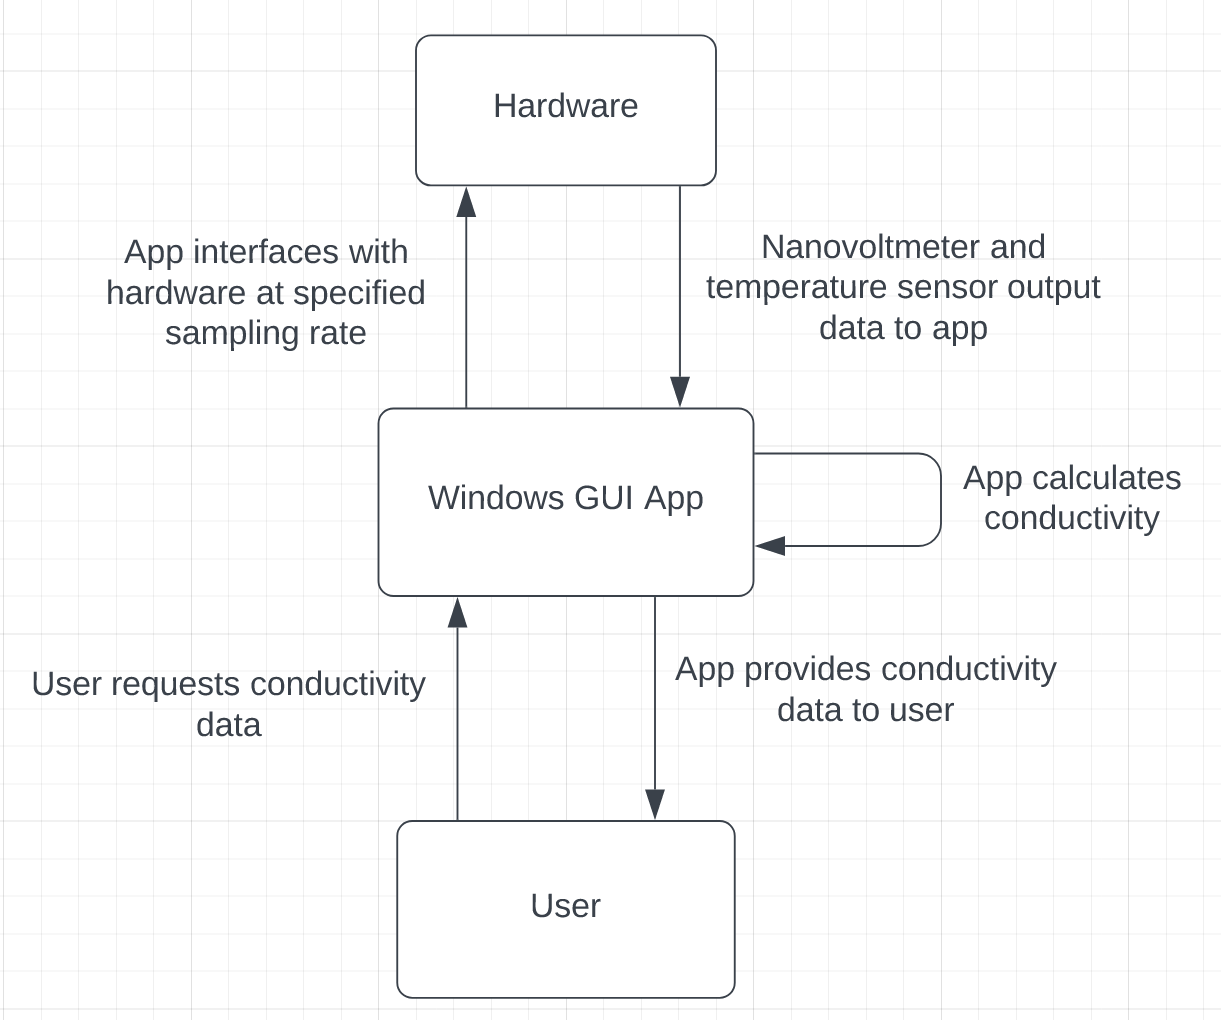
\includegraphics[scale=0.8]{ContextDiagram.PNG}}
\caption{Basic context diagram (subject to change as project progresses)}
\label{fig}
\end{figure}

\subsubsection{Work Partitioning}

\begin{table}[H]
	\centering
	\caption{Work Partitioning}
	\label{my-label}
	\begin{tabular}{|c|c|c|c|}
		\hline
		\textbf{Event \#} & \textbf{Event Name} & \textbf{Input} & \textbf{Output}     \\ \hline
		1 & \begin{tabular}{@{}c@{}}User requests\\conductivity data\end{tabular} & 
            \begin{tabular}{@{}c@{}}Data\\request\end{tabular} & 
            \begin{tabular}{@{}c@{}}Conductivity\\data\end{tabular} \\ \hline
		2 & \begin{tabular}{@{}c@{}}App connects\\to hardware\end{tabular} & 
            \begin{tabular}{@{}c@{}}Data\\sampling rate\end{tabular} & 
            \begin{tabular}{@{}c@{}}Voltage and\\temperature data\end{tabular} \\ \hline
		3 & \begin{tabular}{@{}c@{}}App calculates\\conductivity\end{tabular} & 
            \begin{tabular}{@{}c@{}}Voltage and\\temperature data\end{tabular} & 
            \begin{tabular}{@{}c@{}}Sample\\conductivity\end{tabular}  \\ \hline
	\end{tabular}
\end{table}

\begin{table}[H]
	\centering
	\caption{Work Partitioning - Description}
	\label{my-label}
	\begin{tabular}{|c|c|}
		\hline
		\textbf{Event \#} & \textbf{Description}											\\ \hline
		1 & \begin{tabular}{@{}c@{}}User opens app and requests conductivity data\\for the current sample connected to hardware\end{tabular}	\\ \hline
		2 & \begin{tabular}{@{}c@{}}App interfaces with hardware, sets sampling rate,\\and records data from hardware\end{tabular}	\\ \hline
		3 & \begin{tabular}{@{}c@{}}App uses data received from hardware to calculate\\conductivity of sample\end{tabular}  \\ \hline
	\end{tabular}
\end{table}


\subsubsection{Individual Product Use Cases}

\begin{enumerate}[{UC-}1:]
    
%--Use Case Template
\item Use the App in the lab to measure conductivity changes in sample material\\
    \textbf{Related Requirements:} FR1, FR2, FR3, FR4\\ %Cross reference with requirements below
    \textbf{Initiating Actor:} User\\
    \textbf{Actor's Goal:} Record conductivity changes in sample material during thermal treatment\\
    \textbf{Participating Actors:} User, App, Hardware\\
    \textbf{Pre-conditions:} User in lab; sample material connected to hardware\\
    \textbf{Flow of events for main success:}\\
    $\rightarrow$ 1. User requests conductivity data from App\\
    $\rightarrow$ 2. App interfaces with hardware\\
    $\leftarrow$ 3. Hardware outputs voltage and temperature data to App\\
    $\leftarrow$ 4. App calcaultes and outputs conductivity data to User\\

\item Access the App remotely to monitor conductivity changes in sample material\\
    \textbf{Related Requirements:} FR1, FR2, FR3, FR4, FR5\\ %Cross reference with requirements below
    \textbf{Initiating Actor:} User\\
    \textbf{Actor's Goal:} Monitor conductivity changes in sample material remotely during thermal treatment\\
    \textbf{Participating Actors:} User, App, Hardware\\
    \textbf{Pre-conditions:} User remotely connected to App; sample material connected to hardware\\
    \textbf{Flow of events for main success:}\\
    $\rightarrow$ 1. User requests conductivity data\\
    $\rightarrow$ 2. Request is relayed over network to App\\
    $\rightarrow$ 3. App interfaces with hardware\\
    $\leftarrow$ 4. Hardware outputs voltage and temperature data to App\\
    $\leftarrow$ 5. App calcaultes and outputs conductivity data\\
    $\leftarrow$ 6. Conductivity is relayed over network to User
    
\color{black}
\end{enumerate}

\subsection{Functional Requirements}
% List functional requirements here
\begin{enumerate}[{FR}1.] 
    \item
    The app shall monitor the conductivity of the sample material in real time. 
    \item
    The app shall identify critical changes due to phase transition in the sample.
    \item
    The app shall change the data sampling rate as required.
    \item
    The app shall automate the process of identifying slope changes and correlating these to phase changes in the sample. 
    \item
    The app shall have remote access and control. \\
	
\end{enumerate}

\section{Non-functional Requirements}


\subsection{Look and Feel Requirements}
\begin{adjustwidth}{2.2em}{0pt}
\begin{enumerate}[{NFR-L}1.]
   ADD TEXT
\end{enumerate}
\end{adjustwidth}
 

\subsection{Usability and Humanity Requirements}
\begin{adjustwidth}{2.2em}{0pt}
\begin{enumerate}[{NFR-U}1.]
    ADD TEXT
\end{enumerate}
\end{adjustwidth}

\subsection{Performance Requirements}
\begin{adjustwidth}{2.2em}{0pt}
\begin{enumerate}[{NFR-P}1.]
  % 100/s sampling rate
    ADD TEXT
\end{enumerate}
\end{adjustwidth}

\subsection{Operational and Environmental Requirements}
\begin{adjustwidth}{2.2em}{0pt}
\begin{enumerate}[{NFR-O}1.]
    ADD TEXT
    
\end{enumerate}
\end{adjustwidth}

\subsection{Maintainability and Support Requirements}
\begin{adjustwidth}{2.2em}{0pt}
\begin{enumerate}[{NFR-M}1.]
    ADD TEXT
\end{enumerate} 
\end{adjustwidth}

\subsection{Security Requirements}
\begin{adjustwidth}{2.0em}{0pt}
\begin{enumerate}[{NFR-S}1.]
    ADD TEXT
\end{enumerate}
\end{adjustwidth}

\subsection{Cultural Requirements}
\begin{adjustwidth}{2.2em}{0pt}
\begin{enumerate}[{NFR-C}1.]
    \item The project must not include any graphics or terms that may be considered offensive or inappropriate to the user.\\
    Fit Criterion: To measure this, a usability survey will be conducted to evaluate the graphics and terms on a scale of 1-10. Above 70\% of the surveys returning with a score of 8 will be considered successful.
\end{enumerate}
\end{adjustwidth}

\subsection{Legal Requirements}
\begin{adjustwidth}{2.7em}{0pt}
\begin{enumerate}[{NFR-LR}1.]
    N/A
\end{enumerate}
\end{adjustwidth}

\subsection{Health and Safety Requirements}
\begin{adjustwidth}{2.2em}{0pt}
\begin{enumerate}[{NFR-H}1.]
  % Add item about lab safety  
  \item ADD TEXT HERE
  \item Colours and graphics used in the application should take into account users who may be prone to seizures. \\
    Fit Criterion: There should be no animations that simulate flashing/ flickering (i.e change of brightness or colour at a rapid rate). There should also be no static optical illusions that may simulate amy flashing/ flickering.
    \item Colours should not be too bright, causing potential harm to users eyes. \\
    Fit Criterion: Colours of GUI should be checked to ensure it does not simulate extra light. Example: colours that include the words 'bright,' 'flashy' or 'neon'.
\end{enumerate}
\end{adjustwidth}

\subsection{Installability Requirements}
\begin{adjustwidth}{2.0em}{0pt}
\begin{enumerate}[{NFR-I}1.]
  \item Product requires a Windows computer with the necessary ports to connect to the lab equipment. \\
    Fit Criterion: Run the installation file and install the application successfully. Open the application to see if the readings from the lab equipment are reflected correctly.
\end{enumerate}
\end{adjustwidth}

\section{Project Issues}

\subsection{Open Issues}
% What are some issues we have right now

ADD SOME TEXT HERE

\subsection{Off-the-Shelf Solutions}
The application will use Electron, a JavaScript framework that allows developers to create cross-platform compatible desktop applications. 
Since the use cases of this project are more specialized, there are not many existing solutions available on the market.

\subsubsection{Ready Made Components}
The application will use existing libraries in Electron to further support the communcation with any equipment in the lab.

\subsection{New Problems}
 A potential problem from our product that may arise is the user's ability to learn the software.
  \subsubsection{Potential User Problems}
This product introduces a new learning curve for the user to use the application. 
To minimize this problem, the product will be implemented with a quick start guide and developers will design a user friendly interface.


\subsection{Tasks}
% What do we need to do?
% Communicate lab equipment output to some kind of communication channel (serial port, sockets, named pipes)
% Read data from the communication channel
% Create a GUI that can be installed and run on Windows 7
ADD STUFF HERE 

\subsection{Migration to the New Product}
N/A

\subsection{Risks}
A risk to this project is that the current lab computer uses Windows 7 as its operating system. Although Electron has compatiblity with Windows 7, there appears to be a few issues in the past on GitHub. 
In the case that it does not work, the operating system will have to be upgraded to Windows 10 and the compatibility with the lab equipment is uncertain. Additionally, McMaster University had notified the 
Department of Materials Engineering that Windows 7 is no longer supported but since the lab computer does not require any network connections, it has remained running Windows 7. This poses a future risk of 
the operating system being forcefully upgraded.\\

Another risk is that the lab equipment does not offer the necessary sampling or is not compatible with the lab computer. 

\subsection{Costs}
The largest estimated cost of this project is time. It will require both the developers and the client's time to work and evaluate the project throughout.
Additional expense may be added if additional or new lab equipment is required. 

\subsection{User Documentation and Training}
A main README file will be created and documented for information such as installation, system requirements, and available features. 
An additional safety document will also be created for users, before using any of the lab equipment. 

\subsection{Waiting Room}
ADD STUFF HERE

\subsection{Ideas for Solutions}
ADD MORE STUFF
% Electron
% Serial ports and communication
% Use electron libraries

\bibliographystyle{plainnat}

\bibliography{SRS}

\newpage

\section{Appendix}

N/A

\subsection{Symbolic Parameters}

\begin{itemize}
    \color{red}
    \item \hyperref[sec:sampling]{SAMPLING\_RATE\_PER\_SECOND = 100}
\end{itemize}

\subsection{Reflections}

\noindent Q1: What knowledge and skills will the team collectively need to acquire to successfully complete this capstone project? \\
% Examples of possible knowledge to acquire include domain-specific knowledge from the domain of your application, 
% software engineering knowledge, mechatronics knowledge or computer science knowledge. 
% Skills may be related to technology, writing, presentation, team management, etc. You should look to identify at least one item for each team member.
\noindent Q2: For each of the knowledge areas and skills identified in the previous question, what are at least two approaches to acquiring the knowledge or mastering the skill? 
From the identified approaches, which will each team member pursue, and why did they make this choice?\\

\noindent Response

\end{document}